\section{问题四：救援任务分区与资源配置}

题面要求把 15 个服务区划分为 2 组或 3 组并行开展救援，并明确「各任务组\textbf{分别核算}独立执行所需资源，\textbf{任务执行期间各类资源不得跨组调配}」。这一条把问题从「如何分组更均衡」变成了「分组后还能不能落地」：资源不可跨组复用，意味着每组都必须自备完整的运输与通信保障能力。本节据此建立分区模型、给出完全枚举结果，并如实核算缺口。

\subsection{原子任务单元与完全枚举}

\textbf{不可再拆的原子单元。}分区不能任意切割服务区：若两个服务区在问题三的推荐方案中被同一运输架次访问，则它们在同一组内才能共享那一架次，拆开会使架次方案失效。故先以「被同一架次服务」为边构建服务区之间的必连图，取连通分量为\textbf{原子任务单元}。按问题三联合方案计算，24 个运输架次把 15 个服务区归并为 \textbf{12 个原子单元}（表~\ref{tab:q4-units}），其中 2 个单元（U01、U08）含多个服务区。

\begin{table}[htbp]
	\caption{原子任务单元及其工作量}
	\label{tab:q4-units}
	\centering
	\small
	\begin{tabular}{clcc}
		\toprule
		编号 & 服务区列表 & 运输架次数 & 工作量（h） \\
		\midrule
		U01 & S001, S010, S014 & 5 & 2.6113 \\
		U02 & S002 & 2 & 1.1460 \\
		U03 & S003 & 2 & 1.3072 \\
		U04 & S004 & 3 & 1.6760 \\
		U05 & S005 & 1 & 0.5221 \\
		U06 & S006 & 3 & 1.0677 \\
		U07 & S007 & 3 & 1.4109 \\
		U08 & S008, S011 & 1 & 0.7475 \\
		U09 & S009 & 1 & 0.4335 \\
		U10 & S012 & 1 & 0.5401 \\
		U11 & S013 & 1 & 0.4171 \\
		U12 & S015 & 1 & 0.5083 \\
		\bottomrule
	\end{tabular}
\end{table}

\textbf{完全枚举而非启发式。}12 个单元的分区规模由第二类 Stirling 数给出：$K=2$ 时 $S(12,2)=2047$ 种，$K=3$ 时 $S(12,3)=86\,526$ 种。这一规模仍然完全可以穷举，故本文用受限增长串直接枚举全部非空无序划分（不重不漏，实测枚举数 $2047$ 与 $86\,526$ 均与理论值一致），\textbf{枚举结果即全局最优}，无需迭代搜索。这一条在本题不是可有可无的：下一节将看到，可行分区在全部枚举中一个都不存在，而那正是\textbf{只能靠枚举才能下的结论}——任何单个分区上的缺口核算都无法排除「换个分法就够了」。

\textbf{工作量的口径。}单元的工作量取该单元所含运输架次的飞行器时之和（表~\ref{tab:q4-units}）；而组的工作量还要计入分配给该组的中继飞行器时——分组的意义正在于每组自备完整的运输与通信能力，只算运输侧会低估主力组与小组的差距。故记
\begin{equation}
	W_g=\sum_{p\in \mathcal{P}_g} T_p \;+\; \sum_{k\in \mathcal{K}_g} T^{R}_{k},
	\label{eq:q4-workload}
\end{equation}
其中 $T_p$ 为运输架次 $p$ 的作业时长、$T^{R}_{k}$ 为中继架次 $k$ 从起飞到返航的时长；组间均衡度取变异系数 $CV_W=\sigma(W_1,\dots,W_K)/\bar W$。

为排除单一实现的偏差，本文另用\textbf{组列集合划分整数规划}走第二条路径复核：对每个非空单元子集预生成「组列」，再求恰好 $K$ 组的集合划分最优值。两条路径给出相同的最优资源规模 $R$（$K=2$ 为 31、$K=3$ 为 34），沿用问题一的双路径验证范式。

\subsection{资源需求核算}

对每个任务组，各类资源需求按其\textbf{独立执行时的峰值并发量}核算，而非简单取架次数：

\begin{itemize}
	\item 运输无人机：该组架次占用区间 $[\text{开始},\text{结束}]$ 的重叠峰值，按机型分别统计；
	\item 共享电池：占用区间延伸到充电完成，即 $[\text{开始},\text{结束}+T^{\text{charge}}]$ 的重叠峰值；
	\item 中继无人机：该组所需中继任务的占用区间 $[\text{起飞},\text{返航}+T^{\text{turnover}}]$（周转时间 $300$\,s）的重叠峰值，与 7.4 节中继架次调度的占用口径一致；
	\item 中继能源组件：占用区间取 $[\text{起飞},\text{返航}+\text{充电完成}]$ 的重叠峰值，充电时长按返航 SOC 反算。
\end{itemize}

需要说明的是，若某个中继架次同时服务了属于两个不同任务组的失效区间，则两组\textbf{各配一架}并如实重复计入。这正是分区带来的真实代价，不得为了数字好看而悄悄合并——资源既然不得跨组调配，同一架中继机就不可能同时属于两组。

\begin{table}[htbp]
	\caption{两类分区方案的资源需求}
	\label{tab:q4-partition}
	\centering
	\small
	\begin{tabular}{cccccccc}
		\toprule
		$K$ & 组号 & 服务区数 & A机/B机/C机 & A电/B电/C电 & 中继机 & 中继组件 & 工作量（h） \\
		\midrule
		2 & 组1 & 12 & 4/1/2 & 6/2/4 & 2 & 4 & 15.5822 \\
		2 & 组2 & 3  & 0/1/0 & 0/2/0 & 1 & 2 & 3.4651 \\
		\addlinespace
		3 & 组1 & 10 & 4/1/2 & 6/2/3 & 2 & 4 & 14.8347 \\
		3 & 组2 & 2  & 0/0/1 & 0/0/1 & 1 & 1 & 1.3446 \\
		3 & 组3 & 3  & 0/1/0 & 0/2/0 & 1 & 2 & 3.4651 \\
		\bottomrule
	\end{tabular}
\end{table}

\subsection{分区方案比较与资源缺口}

从资源规模、均衡度与缺口三方面比较两类方案，汇总于表~\ref{tab:q4-compare}。

\begin{table}[htbp]
	\caption{两类分区方案的资源规模、均衡度与缺口}
	\label{tab:q4-compare}
	\centering
	\small
	\begin{tabular}{lcccc}
		\toprule
		$K$ & 枚举分区数 & 最优资源规模 $R$ & 工作量均衡 $CV_W$ & 库存可行分区数 \\
		\midrule
		2 & 2047 & \textbf{31} & \textbf{0.6362} & \textbf{0} \\
		3 & 86\,526 & \textbf{34} & \textbf{0.9045} & \textbf{0} \\
		\bottomrule
	\end{tabular}
\end{table}

\textbf{资源规模与均衡度。}$K=2$ 的最优资源规模 $R=31$、$K=3$ 为 $R=34$，即多分一组要多配 3 件资源。均衡度上，$K=3$ 的 $CV_W=0.9045$ 反而\textbf{大于} $K=2$ 的 $0.6362$——这与「组数越多越均衡」的直觉相反，原因是原子单元的工作量本身极不均匀：最重的 U01 一个单元就占 2.6113\,h，约为最轻的 U11（0.4171\,h）的 6.3 倍，12 个单元合计仅 12.39\,h。在最小化资源规模的目标下，最优解会把大头集中在一组、让小单元各自成组，于是 $K=3$ 把只含一个架次的 U08（S008、S011，0.7475\,h）单独拆成一整组，该组工作量 1.34\,h，均衡度反倒恶化（表~\ref{tab:q4-partition}中 14.83\,h 对 1.34\,h 与 3.47\,h）。这说明\textbf{均衡与省资源在本问题上是一对真实的冲突}，需要按目标选择，而不是默认多分组更好。

\textbf{资源缺口（逐类）。}以库存为基准逐类核算需求与缺口，结果如表~\ref{tab:q4-gap}所示。表中「需求」是\textbf{推荐分区}的需求，按总量口径核算——即全队共用同一份库存时，$K$ 个组各自的峰值需求叠加后有没有超出库存。这是「这套分区能不能落地」的正确判据：资源既然不得跨组调配，每个组占住的机器在它自己的作业期间就归它专用，总量必须逐组相加。要判断某一类缺口是不是分区的必然后果，还要看该类在全部 2047 与 $86\,526$ 个分区上的最小需求（表~\ref{tab:q4-min}）。

\begin{table}[htbp]
	\caption{逐类资源需求、库存与缺口}
	\label{tab:q4-gap}
	\centering
	\small
	\begin{tabular}{lcccccc}
		\toprule
		\multirow{2}{*}{资源类别} & \multicolumn{3}{c}{$K=2$} & \multicolumn{3}{c}{$K=3$} \\
		\cmidrule(lr){2-4}\cmidrule(lr){5-7}
		 & 需求 & 库存 & 缺口 & 需求 & 库存 & 缺口 \\
		\midrule
		A 型运输无人机 & 4 & 4 & 0 & 4 & 4 & 0 \\
		B 型运输无人机 & 2 & 2 & 0 & 2 & 2 & 0 \\
		C 型运输无人机 & 2 & 2 & 0 & 3 & 2 & \textbf{1} \\
		A 型共享电池   & 6 & 6 & 0 & 6 & 6 & 0 \\
		B 型共享电池   & 4 & 4 & 0 & 4 & 4 & 0 \\
		C 型共享电池   & 4 & 4 & 0 & 4 & 4 & 0 \\
		中继无人机     & 3 & 2 & \textbf{1} & 4 & 2 & \textbf{2} \\
		中继能源组件   & 6 & 6 & 0 & 7 & 6 & \textbf{1} \\
		\bottomrule
	\end{tabular}
\end{table}

\begin{table}[htbp]
	\caption{全部分区中的最小需求：区分推荐分区的缺口与结构性缺口}
	\label{tab:q4-min}
	\centering
	\small
	\begin{tabular}{lcccccc}
		\toprule
		\multirow{2}{*}{资源类别} & \multicolumn{3}{c}{$K=2$（2047 个分区）} & \multicolumn{3}{c}{$K=3$（$86\,526$ 个分区）} \\
		\cmidrule(lr){2-4}\cmidrule(lr){5-7}
		 & 最小需求 & 库存 & 最小缺口 & 最小需求 & 库存 & 最小缺口 \\
		\midrule
		A 型运输无人机 & 4 & 4 & 0 & 4 & 4 & 0 \\
		B 型运输无人机 & 2 & 2 & 0 & 2 & 2 & 0 \\
		C 型运输无人机 & 2 & 2 & 0 & 2 & 2 & 0 \\
		A 型共享电池   & 6 & 6 & 0 & 6 & 6 & 0 \\
		B 型共享电池   & 4 & 4 & 0 & 4 & 4 & 0 \\
		C 型共享电池   & 4 & 4 & 0 & 4 & 4 & 0 \\
		中继无人机     & 2 & 2 & 0 & 3 & 2 & \textbf{1} \\
		中继能源组件   & 4 & 6 & 0 & 4 & 6 & 0 \\
		\bottomrule
	\end{tabular}
\end{table}

\textbf{核心结论：按题目「资源不得跨组调配」的规则，$K=2$ 与 $K=3$ 在现有库存下均不可行。}2047 个与 $86\,526$ 个分区中，满足总量口径资源约束的分区数为 \textbf{0}。但两者不可行的成因\textbf{并不相同}，需要分开说清楚——把两种成因混为一谈会得出过强的结论：

\begin{enumerate}
	\item \textbf{$K=3$ 的中继无人机是\textbf{结构性}短缺。}题目要求资源不得跨组调配，则每个非空任务组都必须自备通信保障能力；本算例的 19 个失效区间遍布各组，故\textbf{每个非空组至少要占 1 架中继无人机}。$K=3$ 有 3 个非空组，全部分区中继无人机总需求的最小值就是 $3$，而库存只有 $2$ 架（表~\ref{tab:q4-min}「中继无人机」行最小缺口 $1$）。这一架缺口\textbf{与怎么分组无关}：只要分成 3 个都含失效区的组，就必然短缺一架，枚举 86\,526 个分区也躲不掉。
	\item \textbf{其余各类在 $K=2$、$K=3$ 下都不是结构性短缺。}把每一类资源单独拿出来看它在全部分区上的最小需求（表~\ref{tab:q4-min}），除 $K=3$ 的中继无人机外，其余各类（含 $K=2$ 的中继无人机）的\textbf{最小缺口均为 0}：A 型运输无人机最小只需 4 架、B 型与 C 型运输无人机各 2 架、三类共享电池的最小需求分别为 6/4/4 组、中继能源组件 4 个——每一项都\textbf{不超过库存}。也就是说，单独针对这些类别中的任何一类，都存在一个不超库存的分区。$K=2$ 时中继无人机的最小需求恰为 2 架、正好等于库存，正是上述「每组一架」机制的临界情形。
	\item \textbf{第二重来源：联合约束。}对 $K=2$，不可行性无法归因于任何单类短缺（第 2 条），故只能来自联合约束：由第 2 条与「可行分区数为 0」可直接推出，\textbf{不存在任何一个分区能同时取到八类资源各自的最小值}——若存在，该分区各类需求就都等于对应最小值、都不超库存，它本身就会是一个可行分区，与枚举结果矛盾。于是「逐类看处处有余量」与「整体看无一处可行」并存。$K=3$ 则是两种成因叠加：中继无人机的结构性缺口已足以判定不可行，联合约束在此之外仍然存在。
	\item \textbf{推荐分区的缺口是「省资源＋求均衡」这一目标的代价，但其中一部分消不掉。}按 $R$ 最小、$CV_W$ 次小选出的推荐分区（表~\ref{tab:q4-partition}）需要：$K=2$ 缺中继无人机 1 架，合计 1 件；$K=3$ 缺 C 型运输无人机 1 架、中继无人机 2 架、中继能源组件 1 件，合计 4 件。$K=2$ 的那一件与 $K=3$ 的非中继部分\textbf{可以分别}靠换一个分区消去（表~\ref{tab:q4-min} 中相应类别都有取到库存水平的分区），但\textbf{不能同时}消去（第 3 条）；而 $K=3$ 中继无人机缺口中的那 1 架是结构性的（第 1 条），\textbf{换任何分区都消不掉}。
\end{enumerate}

\textbf{与「分区放大需求」这一直觉的关系。}分组推高需求的机制是各组峰值叠加：某类资源在单个组内的峰值也许远小于库存，但 $K$ 组同时作业时占用之和仍可能超过那一份共享库存。本算例的枚举表明，这个效应在 $K=2$ 时确实\textbf{不足以}构成任何单类资源的结构性缺口，但在 $K=3$ 时对中继无人机\textbf{恰好越过了临界点}——因为中继无人机库存只有 2 架，而「每组一架」的下界随组数增长，$K=3$ 时 $3>2$。把这一条与联合约束混为一谈，会得出「$K=3$ 也只是联合约束问题」的过强结论，本文不作此表述。

\textbf{落地建议。}按题意「资源不得跨组调配」的硬判据，两类分区在现有库存下都不可行，且完全枚举证明这\textbf{不是换一种分法就能回避的}（可行分区数为 0）。因此：

\begin{itemize}
	\item 若必须分区，就需要扩充机队，扩充清单取决于所选分组数与分区。按推荐分区计：$K=2$ 需补中继无人机 1 架；$K=3$ 需补 C 型运输无人机 1 架、中继无人机 2 架、中继能源组件 1 件。其中\textbf{$K=3$ 的中继无人机缺口有 1 架是结构性的}，无论改选哪个分区都必须补；其余各项若愿意牺牲资源规模 $R$ 与均衡度 $CV_W$，可改选缺口更小的分区，但不可能降到 0。
	\item 若不扩充机队，更现实的结论是\textbf{不分区}：以问题三的单组联合方案整体执行，其资源需求不超过现有库存（8 架运输无人机与 14 组共享电池全部投入周转，见 6.4 节），而分区虽然在调度视角上便于并行，却在本题「资源不得跨组调配」的规则下不可行。
\end{itemize}

图~\ref{fig:q4-resource}以雷达图与缺口柱状图并列展示两类方案在八类资源上的需求分布与缺口构成；图~\ref{fig:q4-partition}则给出原子单元之间的必连关系、各单元工作量的空间分布以及两类分区下的资源规模分布。

\begin{figure}[htbp]
	\centering
	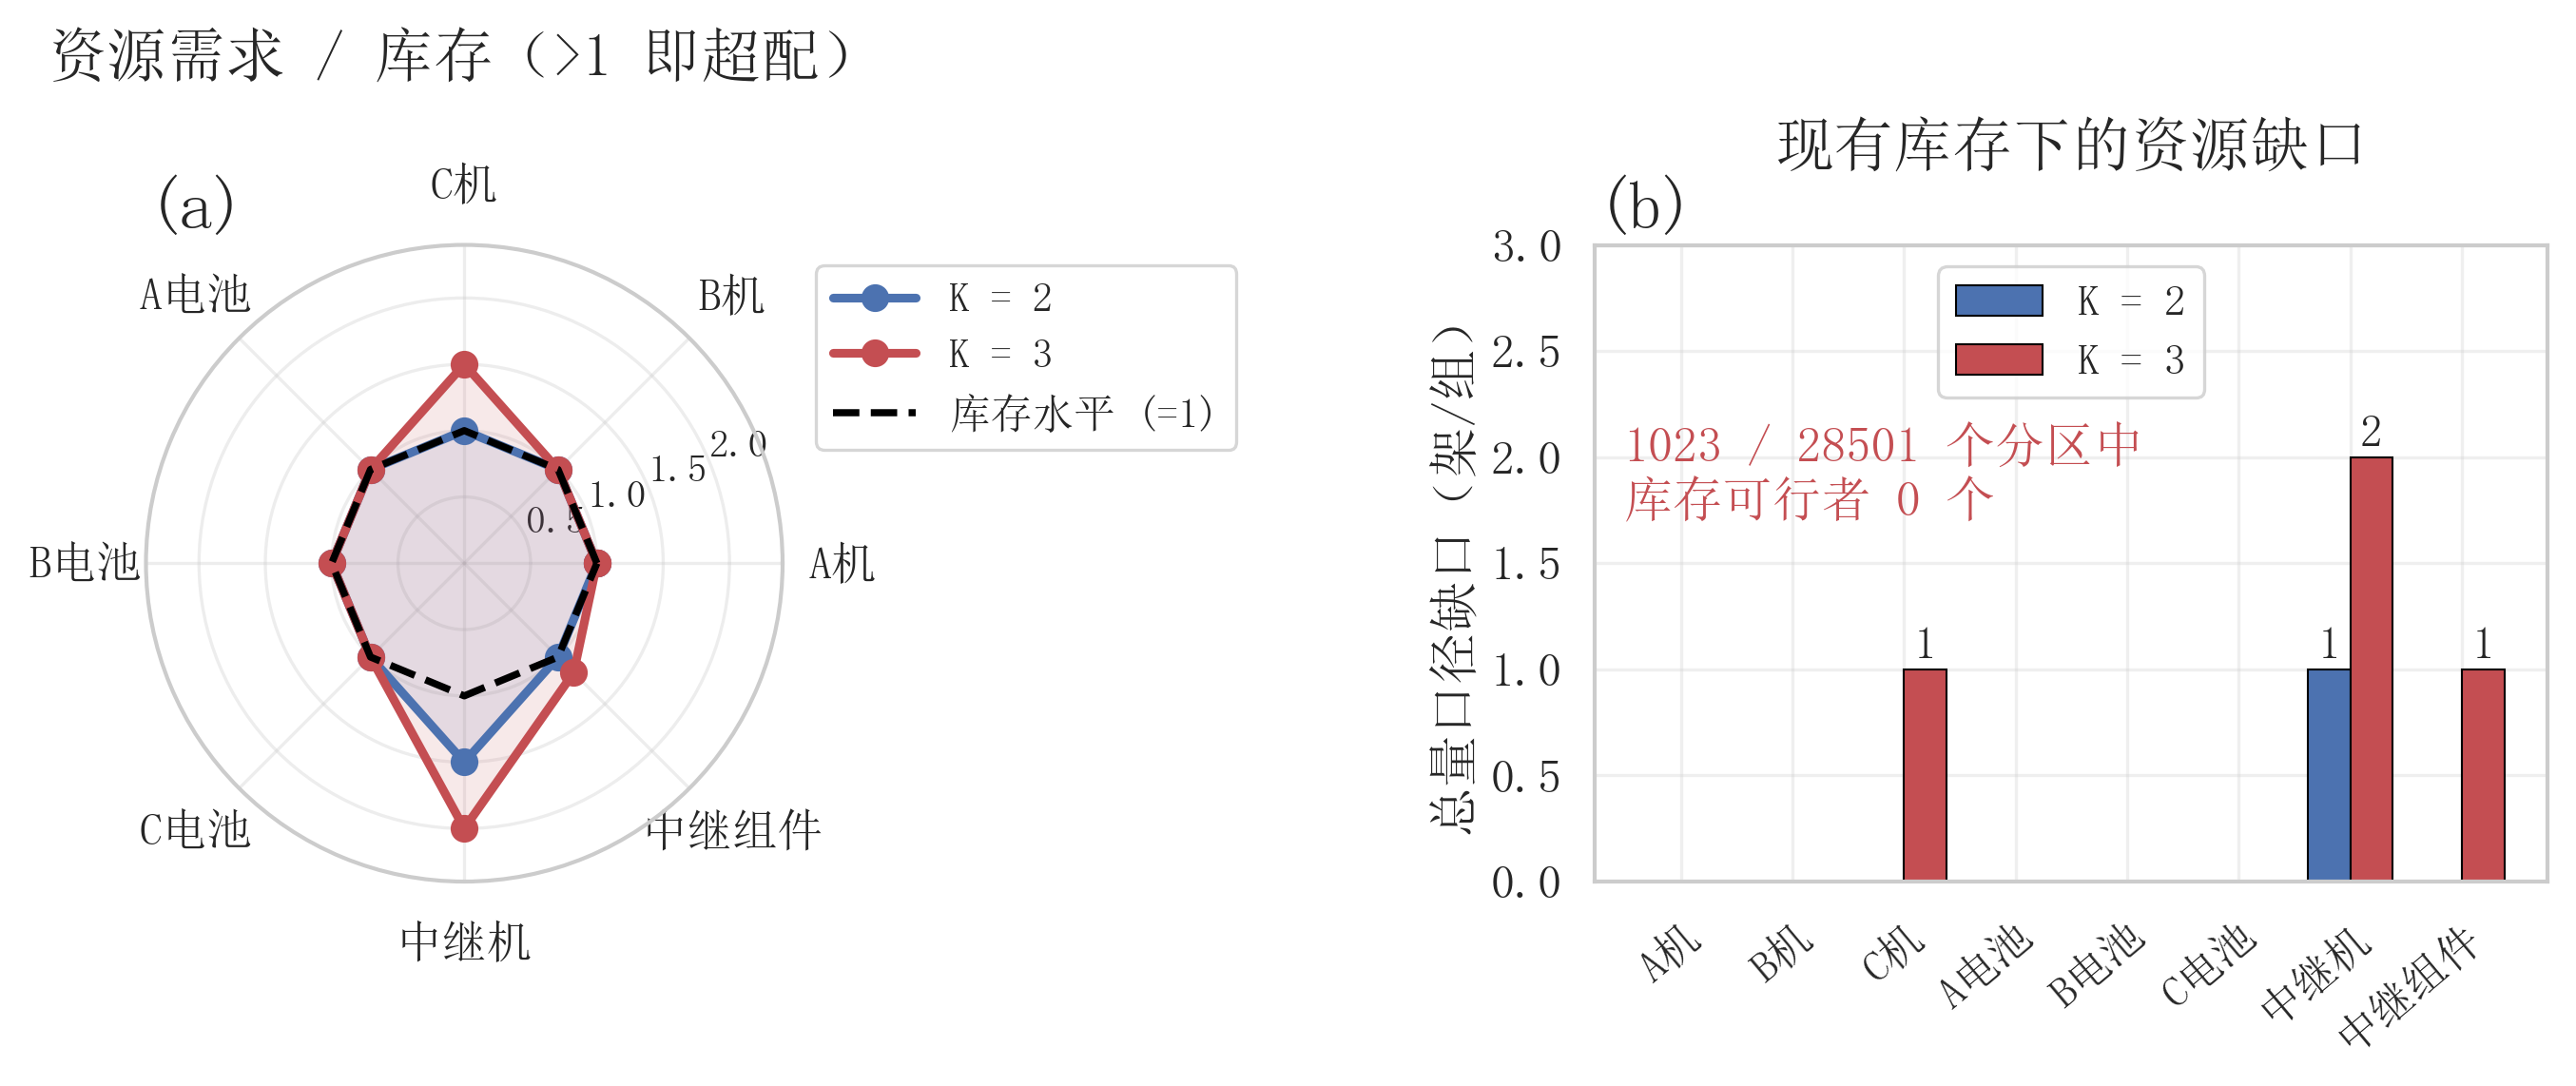
\includegraphics[width=0.95\textwidth]{figures/fig_q4_resource.png}
	\caption{两类分区的资源需求与缺口}
	\label{fig:q4-resource}
\end{figure}

\begin{figure}[htbp]
	\centering
	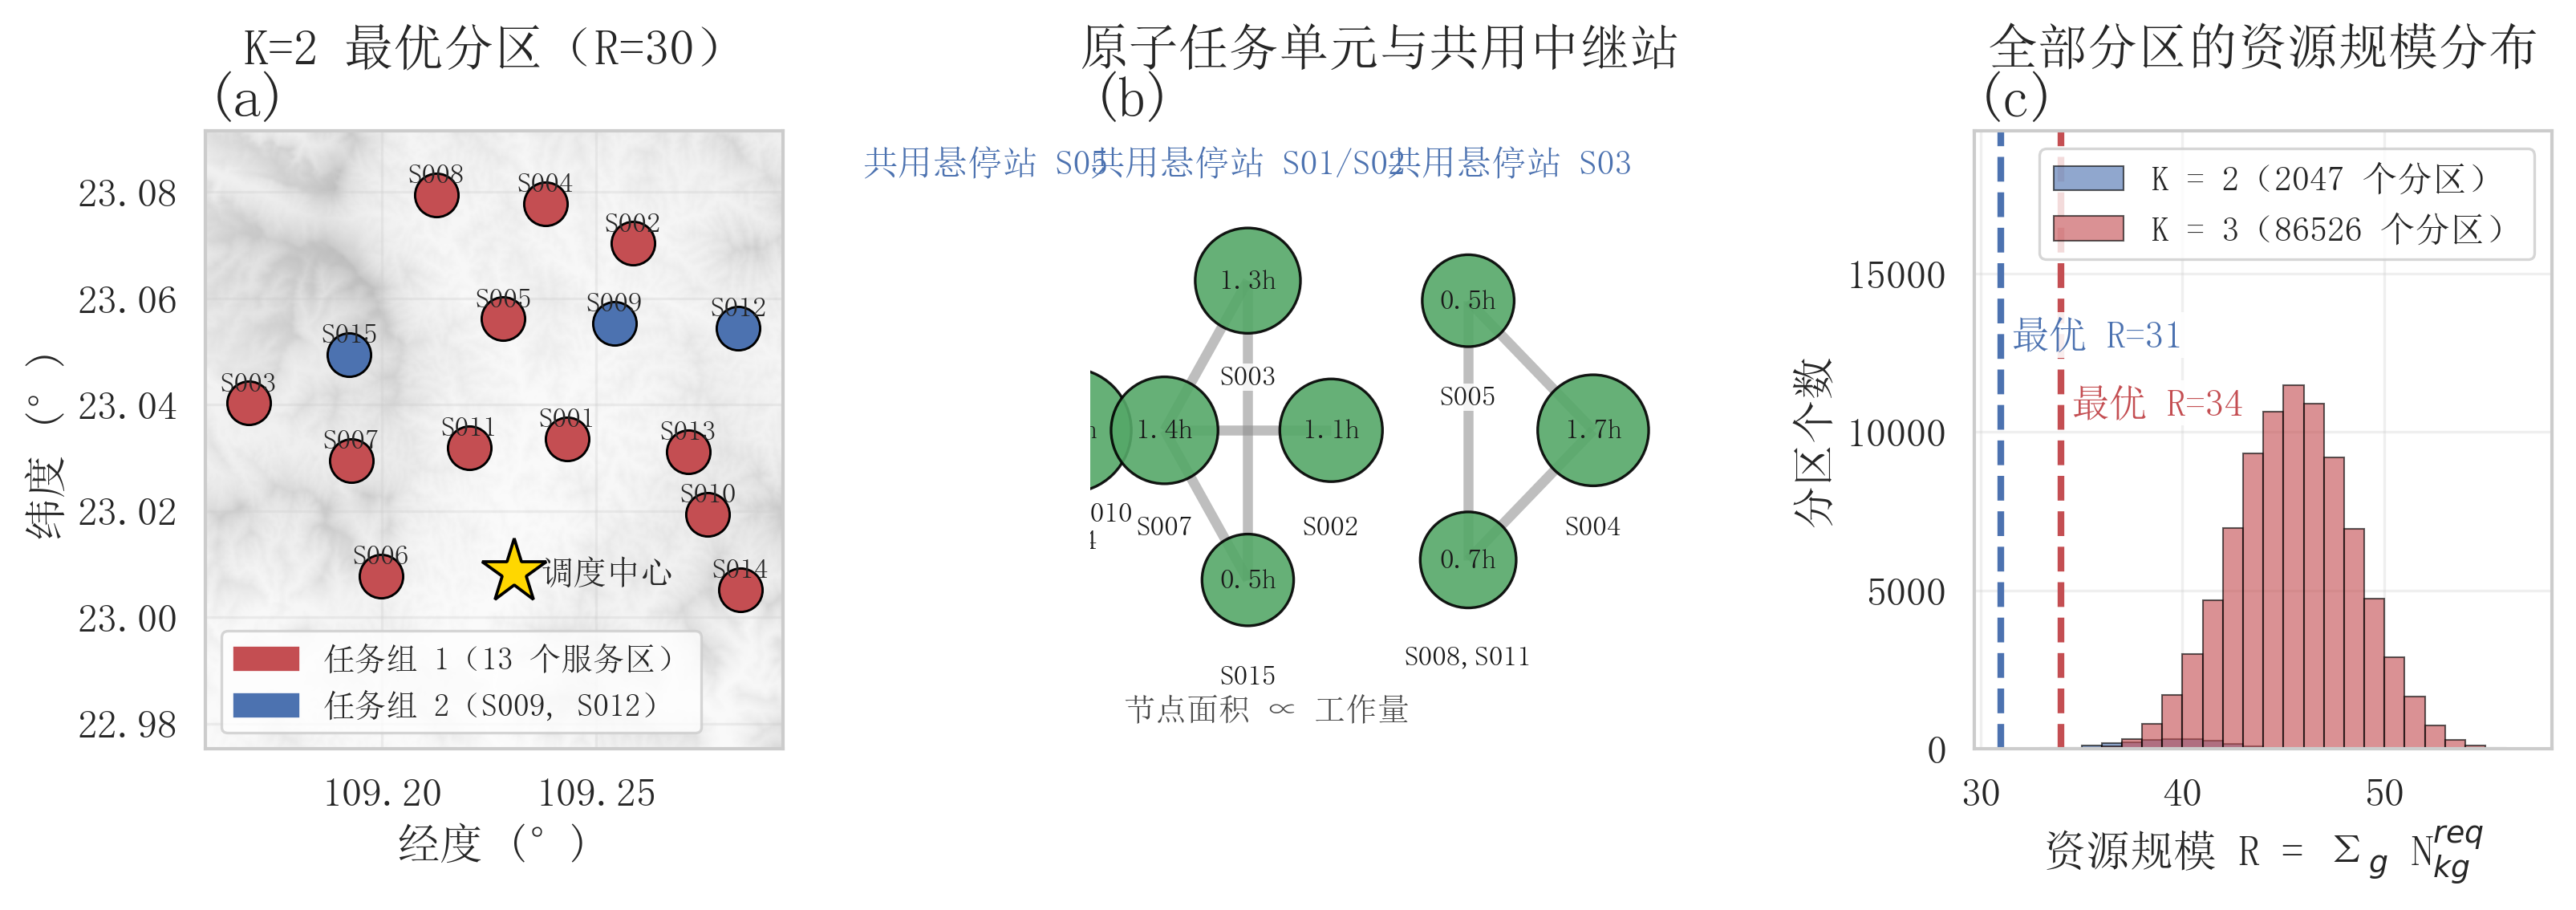
\includegraphics[width=0.95\textwidth]{figures/fig_q4_partition.png}
	\caption{原子任务单元与两类分区资源分布}
	\label{fig:q4-partition}
\end{figure}
